
\section{The Phase II Project}
\label{sec:phaseII}
%% {\em Provide an explicit, detailed description of the Phase I research
%%   approach and work to be performed.  Indicate what will be done, by
%%   whom (small business, subcontractors, research institution, or
%%   consultants), where it will be done, and how the work will be
%%   carried out.  If applicant is making a commercial or in-kind
%%   contribution to the project, please describe in detail here.  The
%%   Phase I effort should attempt to determine the technical feasibility
%%   of the proposed concept which, if successful, would provide a firm
%%   basis for the Phase II grant application.

%%   Relate the work plan to the objectives of the proposed project.
%%   Discuss the methods planned to achieve each objective or task
%%   explicitly and in detail.  This section should be a substantial
%%   portion of the total grant application.} 

\subsection{Technical Objectives}
%% {\em State the specific technical objectives of the Phase I effort,
%%   including the questions it will try to answer to determine the
%%   feasibility of the proposed approach.}

The requirements being addressed include the development of a robust framework 
for in-situ verification and validation in general purpose numerical simulation 
packages. In particular, the objective of this project is to address the need
for tools that automate verification of end-user numerical solutions in the 
NEAMS toolkit. The Phase II project will meet this need by developing a framework
that facilitates the creation of explainable numerical simulations that produce
a final solution \emph{and} a detailed report on why that solution should be trusted.

Toward this goal, RNET Technologies and ORNL will pursue the following objectives:

\begin{enumerate}

\item \rnetprop{Harden and extend the prototype developed during phase I. In particular, the phase II effort 
will focus on developing more robust mechanisms for specifying injection points inside existing code bases. }
\item \rnetprop{Develop mechanisms for efficient in-situ comparisons between data in a distributed environment. In-situ comparison of variables with experimental and/or analytical results will significantly reduce the amount of IO required in \VV testing, while also providing a fine grained mechanism for detecting at what point a solution diverges from
the expected result.}
\item \rnetprop{Minimize execution times through job based parallelism. This will shift the burden
of V\&V testing out of the main simulation, allowing for faster runtime, especially for testing methods that require the same function to be executed multiple times.}
\item \rnetprop{ Develop a robust set of generic \VV tests. The development of these tests (e.g., mesh refinement studies, the method of manufactured solutions, sensitivity analysis, uncertainty quantification) will equip the users with the tools required to perform end-user \VV.}
\item \rnetprop{Demonstrate the value of the VnV framework as a component in the NEAMS tool-chain (MOOSE, libMesh and PETSc). Integration into these tools will answer the NEAMS call for tools that support end-user verification
of numerical simulations. Integration into the NEAMS workbench will provide access to the tools in the seamless manor users of the workbench have come to expect. } 

\end{enumerate}

\subsection{Work Plan}
\label{sec:workplan}

The goal of the Phase II project will be to develop a fully functional, efficient, battle tested framework 
for integrating advanced end-user verification and validation into general purpose numerical simulation packages. In what follows, we outline the work required to achieve this goal. 

\subsubsection{Hardening and Optimization of the Injection Point System}

The injection point system developed during Phase I relies on C style Macros and string based pointer casts. In a \emph{trusted} environment, this is an efficient (void* casts are almost free) and portable (it is written in C)  approach. However, there are three main weaknesses need to be addressed prior to production:

\begin{itemize}
 \item {\bf String based pointer casts:} The system developed in Phase I uses developer provided strings to infer the type of each variable. Under the hood, the injection point system uses these strings to ensure compatibility between test parameters and injection point variables. The key issue is that the strings specified at each injection point cannot be verified during compilation. This will causes issues in cases where, say, the developer changes the type of a variable, but forgets to update the type string in the injection point declaration.  
  
 \item {\bf Restrictive type specifications:} The current system uses C compliant pre-processor macros to simplify the process of describing injection points and variables. The benefit of this approach is that the injection points can be compiled into any application without significant changes to the build system. The downside is that the single-pass, text based pre-processing supported by the C preprocessor places a significant restriction on the functionality that can be imparted.
 
 \item{\bf Constant Correctness} The current system provides the testing algorithms with direct access to the data structures and variables specified at each injection point. This access allows for efficient, unrestricted testing of the data structures. There are some exciting use cases for this functionality (parallel debugging, computational steering, etc.); however, from the perspective of V\&V, it is imperative that testing routines do not alter the trajectory of the simulation in any way.  
\end{itemize}
 
In Phase II, the project team will investigate and develop an annotation based system for defining injection points. This annotation system will provide users with full control over what variables can be accessed at each injection point, including the ability to provide access to internal components of data structures, describe the domain decomposition of distributed arrays and to complete pre-test processing. The annotation system will also provide a mechanism for injection point detection in non-object orientated programming languages where runtime injection point detection cannot be completed. However, the primary benefit of this new system will be that it will automatically detect the type of the variables tagged for inspection at each injection point.  

To implement this annotation system, the project team will create a set of custom pre-processor directives (i.e., pragmas) using Clang. Clang is a compiler front end for the C family of languages. It is a well supported, well documented compiler package designed as a drop in replacement for GCC. We we utilize Clangs library API for implementing custom Pragma routines to implement a pre-processor that transforms the annotations into valid injection point specifications. 

To address the issues with constant correctness, the team will develop support for fine-grained regression testing. This functionality will allow users to track the progress of a simulation against a VnV output file that was generated without significant testing. This will allows users to compare the current state of the simulation against an expected result at every level of the simulation. 

\subsubsection{Efficient Statistical Comparisons in Distributed Settings} 

One of the major benefits of the VnV framework is that the tests are executed inside the simulations distributed environment. This allows for the development of efficient, parallel testing algorithms. To capitalize on this functionality, the Phase II effort will include an investigation into efficient statistical methods for analyzing, asserting and comparing data stored in distributed arrays. 

The first step toward working with distributed arrays is to obtain some information about the global partition of the data. This information is readily available in simulations that use regular data decompositions (i.e., block, cyclic,etc.), but it is not generally known in simulations where the data is distributed irregularly across the processors. Such irregular decompositions of data are common in applications that support mesh refinement, but not load balancing. 

The naive approach to determining the global partition is to explicitly form the partition using global MPI communication. This is a robust approach that will be immediately applicable in a large number of situations. However, the large storage cost required to build the global partition (O(P), where $P$ is the number of processors) is likely to become an issue in peta- and exa-scale environments \cite{hypre-assumed}. 

To that end, the Phase II effort will include a detailed analysis of the optimal algorithms for forming the global partition in a distributed setting. This will include the implementation and profiling of the aforementioned naive approach, as well as an investigation into more advanced approaches parallel rendezvous algorithms such as forming a hash based distributed directory \cite{hpre-nine} and the assumed partition algorithm \cite{hypre-assumed}. 

The second step will be to develop efficient algorithms for comparing and analyzing distributed data based on that partition. This will include the development of the VnV Testing suite for distributed Arrays. This testing suite will include a variety of analysis routines for analyzing data including, means, std deviation, variance, co-variance, etc. A collection of functions implementing matrix based metrics will also be included (e.g., one norms, symmetry, positive definiteness, etc). 

A key goal of the Phase II effort will be to develop support for comparing solutions obtained in distributed arrays with data stored on disk. This will be achieved using the ADIOS2 read-write API. In this case, the global partition determined above will be used in conjunction with ADIOS to distribute the correct data to each processor. The project team will then perform a detailed analysis of existing third party data transfer and interpolation tools to determine the best approach to efficiently comparing experimental data with the data in the distributed arrays. 

\subsubsection{Reducing Run-times with Job Parallelism}

Performing \VV tests in a distributed environment will be expensive, both computationally and due to the data movement required to deal with the domain decomposition employed by the application. To address this problem, the VnV toolkit will support the offloading of tests to external processes. This functionality will allow for speedup through job parallelism for expensive testing routines like sensitivity analysis and mesh refinement, while also allowing for specific tests to be run on the optimal architecture (e.g., an test involving image processing could be offloaded to a GPU enabled architecture).  

The first step toward supporting test offloading will be to implement an effective mechanism for transferring the required 
data from the simulation to the external testing processes. To do this, the project team will use the ADIOS 2 Sustainable Staging Transport (SST). The SST is a classic streaming data architecture that allows for direct connection between data produces and data consumers. 

The VnV toolkit will use the SST engine to stream the required testing data to a VnV Testing Manager. The test manager will determine the best available resource for running the given test and launch the job. To do this, the test manager will utilize the extensive support for integrating with remote job schedulers available in the Eclipse Parallel Tools Platform (PTP). 

The PTP project provides an integrated development environment to support the development of parallel applications written in C, C++, and Fortran. Eclipse PTP provides; support for the MPI, OpenMP and UPC programming models, as well support for a wide range of batch systems and runtime systems, including PBS/Torque, LoadLeveler, GridEngine, Parallel Environment, Open MPI, and MPICH2.

In this case, PTP provides a simple interface for launching tests as separate processes. The open research question to be answered during the Phase II effort is to determine in which situations test offloading is beneficial. In particular, the project team will look to implement heuristic algorithms that detect when the cost of streaming the required testing data outweighs the performance benefits associated with offloading the tests. 

\subsubsection{Integrate Third Party Tools for Mesh Refinement, UQ and Sensitivity Analysis.}

Mesh refinement studies, uncertainty quantification (UQ) and sensitivity analysis (SA) are all essential components of a robust \VV regimen. To that end, the Phase II effort will include the development of a VnV testing library that integrates with third party tools to facilitate testing using these approaches.  

UQ and SA will be developed using DAKOTA. DAKOTA provides a set of black-box tools for performing parameter optimization, UQ 
and SA. The Phase II effort will include the development of a flexible interface for setting up and running DAKOTA tools at injection points, and the development of the output templates for displaying the results. Most high performance finite element packages support some level of adaptive mesh refinement (e.g., libMesh, Fenics, MFEM, etc.), hence, rather than trying to patch in third party tools, the mesh-refinement tool will be developed as a generic interface for interacting with existing mesh refinement functionality. 

\subsubsection{Integration with NEAMS tools and the NEAMS workbench} 

To demonstrate the value of the VnV framework, the project team will integrate the VnV framework into the open-source components of the NEAMS tool-chain (PETSc, libMesh and MOOSE). Doing so will provide ample opportunities for testing, while also allowing us to demonstrate the performance of the toolkit in real codes with real applications. Moreover, this integration will provide a road map for integration into MOOSE based NEAMS applications like BISON. 

Integration into NEAMS tool-chain will be a three step process:

\begin{itemize}
 \item The first step will be to insert injection points into key locations in the MOOSE, libMesh and PETSc source codes. The optimal locations for inserting these injection points will be determined after detailed profiling of example codes; however, some options include during each linear solver iteration, during each nonlinear iteration, during finite element matrix construction (if it exists) and inside the function for calculating the action of the Jacobian
 on a vector (for matrix free problems). 
 
 \item The second step will be to allow users to configure the VnV testing directly in the MOOSE input file using the MOOSE input file syntax. This will provide users of MOOSE with a seamless mechanism for setting up and running tests. This will involve writing a custom MOOSE action for setting up and configuring the VnV runtime module.
 \item The third step will be to enable context-aware auto-complete for MOOSE based VnV configuration files in the NEAMS workbench. The workbench has integrated support for extracting the information required to setup input file verification and auto-complete from MOOSE applications; however, there will likely be some additional work required to correctly setup this up for tests stored in external libraries. In particular, the current system requires that the tests adhere to a specific XSD specification, but there is not yet a system for extracting the exact parameters required to inject a specific test. 
 \item The last step will be to provide support for viewing the final VnV reports in the NEAMS workbench. The project team demonstrated how the QWebEngineView can be used to display the HTML VnV report in a QT window. The Phase II effort will extend that demonstration by providing the callback function required to interact with the NEAMS workbench interface (menus, docs, etc).
\end{itemize}

\subsection{Performance Schedule and Task Plan}
\label{sec:taskplan}

% Use wrapfigure here instead?
\begin{wrapfigure}{r}{0.5\linewidth}%[thb]
%\begin{figure}[thb]
\begin{center}
\leavevmode
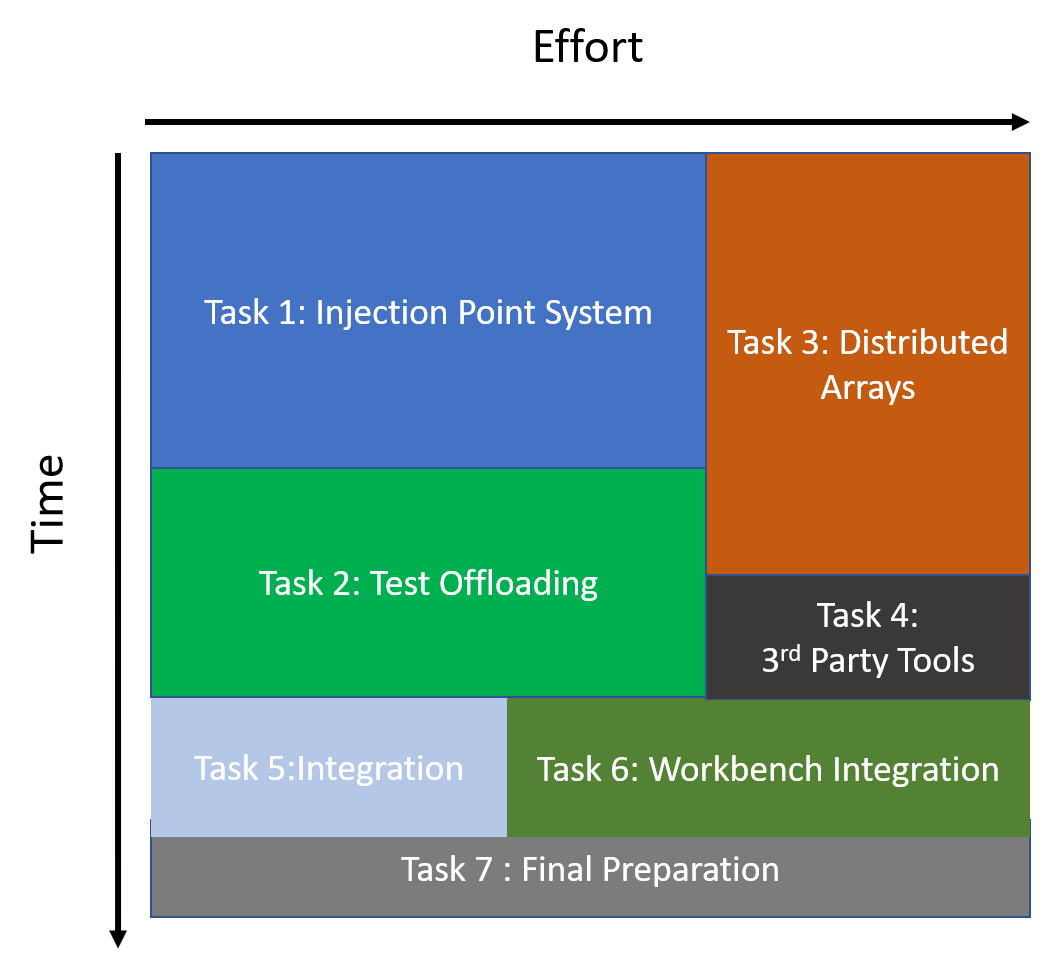
\includegraphics[width=1.0\linewidth]{./narrative/figures/tasks.png}
\end{center}
\caption{Overview of task dependencies and timeline.}
\label{fig:tasks}
\end{wrapfigure}

RNET would like to present the project ideas and research plan to the
DOE Program Manager and other interested scientists. The meeting will
be used to discuss features and to identify the specific NEAMS applications and computer
resources that will benefit from this project.  This meeting will be
scheduled soon after the Phase II contract is awarded. The meeting can
be hosted at RNET, a DOE site suggested by the Program Manager or via
a teleconference.

RNET will submit all reports as required by the contract (e.g., annual reports, 
a continuation report, summary reports, and a final report) to the DOE program 
manager and other interested DOE scientists.

The research and development topics described in Section~\ref{sec:workplan} 
will be addressed by the tasks described in the remainder of this section. Most 
tasks require active collaboration between RNET and ORNL. 
Figure~\ref{fig:tasks} summarizes at a high level the dependencies among tasks and
approximate anticipated task durations. The duration of the Phase II 
project is 104 weeks. Specific details are included in the description of each 
task.


\newcounter{taskCount}
\setcounter{taskCount}{0}

\refstepcounter{taskCount}\label{task:2.5}
\subsubsection{Task \ref{task:2.5}: Development of the Annotation based Injection Point System  }

\rnetprop{In this task, the project team will develop the Annotation system for specifying injection points and describing injection variables. This will include the development of
the custom LLVM compiler extensions required to process these annotations. At the end of this task, users will be able to specify injection points and injection point variables using either the new Annotation point system, or using the more portable, but less robust Phase I approach. 

To test the Annotation based injection point system, the project team will write injection points at several key locations in the MOOSE software stack, including inside the source code of several MOOSE modules, the core MOOSE framework, libMesh and PETSc. This will allow us to demonstrate the cross-library potential of the Annotation based system, while also acting as the first step toward integration of the tools a number of the NEAMS tools.}

\rnetprop{
RNET will work on the implementation for this task and ORNL will provide inputs and guidance.
}


\refstepcounter{taskCount}\label{task:3}
\subsubsection{Task \ref{task:3}: Develop methods for offloading tests to external processes. }

\rnetprop{In this task, the project team will add support for test offloading using the ADIOS2 SST architecture. This will include the development of the VnV test manager and integration with the PTP platform, a task which will likely involve custom modifications to the PTP platform. Once implemented, test offloading will be tested using the VnV enabled MOOSE software stack developed in Task~\ref{task2.5}. The goal of this task will be to see a significant speedup when using test offloading over the standard in-situ testing routines. }

\rnetprop{
RNET will work on the implementation for this task with ORNL providing assistance with ADIOS and any modifications to PTP.
}

\refstepcounter{taskCount}\label{task:23}
\subsubsection{Task \ref{task:23}: Development of efficient statistical \VV tools for distributed arrays.}

\rnetprop{In this task, the project team will investigate the optimal approaches for conveying information about the data decomposition. This will involve robust analysis of three approaches to determining the global partition; explicitly forming the global partition; building a distributed directory; and using an assumed partition algorithm. This task will also include the development of a number of efficient statistical tools for asserting the state of the data in distributed arrays.

At the completion of this task, users will be able to efficiently compare and analyze distributed arrays using the VnV framework. To test these implementations, the project team will set up tests for performing assertions on various PETSc vectors and matrices. This testing will compare the performance of each of the global partition methods and each of the analysis tools.} 

\rnetprop{
RNET and ORNL will collaborate on this task.
}

\refstepcounter{taskCount}\label{task:22}
\subsubsection{Task \ref{task:22}: Development of Generic tools for Mesh refinement, Uncertainty quantification and Sensitivity Analysis.}
\rnetprop{In this task, RNET will implement generic \VV tools for mesh refinement, uncertainty quantification and sensitivity analysis. In the case of mesh refinement, the approach taken will be to create a generic interface for interacting with the automatic mesh refinement functionality that already exists in finite element libraries like LibMesh and Fenics. The overall goal is to create a generic VnV test that can be attached to the main function of the executable such that it automates the process of running mesh refinement and mesh convergence studies. In the case of UQ and SA, the project team will develop an interface for specifying the tools available in DAKOTA as VnV tests. }

\rnetprop{
RNET will be responsible for this task with ORNL providing input and guidance.
}


\refstepcounter{taskCount}\label{task:1}
\subsubsection{Task \ref{task:1}: Integration into the NEAMS tool-chain}
\rnetprop{
  In this task, the program team will integrate the VnV framework into a variety of real applications. Initially, this 
  testing will be completed in tools used heavily in the NEAMS toolkit; MOOSE, libMesh and PETSc, but other third party 
  applications will also be investigated. To ensure seamless integration with the MOOSE tools, the project team will re-implement the XML based configuration file using the MOOSE input file format. This will allow for the configuration of the VnV tests in   a MOOSE application directly from the input file.
  
  The goal of this task will be to generate informative, production quality VnV 
  reports for a number of examples available in the MOOSE testing suite. Doing so allows us
  to test every facet of the proposed framework, while also acting as the first demonstration of the
  value provided by the framework. These results of these tests will be hosted on the RNET website 
  as they become available. 
}

\rnetprop{
RNET will be responsible for this task and ORNL will provide guidance on various technical implementations and details.
}
\refstepcounter{taskCount}\label{task:11}
\subsubsection{Task \ref{task:11}: Development of an interface for the NEAMS workbench}
\rnetprop{
  In this task, the project team will integrate the toolkit directly into the NEAMS workbench. This will be
  a two stage process. First, the project team will implement the required interface files for enabling 
  the context aware auto-complete features available in the NEAMS workbench. MOOSE based input files are already largely supported in the workbench; however, there will likely be some issues with determining which tests are applicable at which 
  injection points. Second will be create the interfaces for viewing the HTML based VnV reports inside the QT based workbench. As demonstrated in Phase I, this will be completed using the QWebEngineView components support for displaying HTML files inside QT windows. 
}

\rnetprop{ 
RNET will be responsible for this task
}

\refstepcounter{taskCount}\label{task:4}
\subsubsection{Task \ref{task:4}: Preparation for the First Release }
\rnetprop{In this task, the project team will prepare the package for its first release. This will include writing documentation ,user manuals and tutorials. 

An important goal of this task will be to develop a mechanism for reducing the size of the VnV reports. In particular, this task will involve modifying the report generation system such that it maximizes data reuse in situations where an injection point or test is encountered multiple times within a simulation. Support for lazy-loading of content in collapsed sections will also be implemented. Such features are not critical to the functionality of the toolkit; however, they will significantly improve the usability of overall product. The custom markdown format will also be hardened, extended and released as part of this task. }

\rnetprop{
RNET will work on the implementation for this task
}


\subsection{Facilities/Equipment}
\subsubsection{RNET Facilities}
RNET has the necessary office equipment to manage an SBIR/STTR contract
including networks, workstations, and accounting software. In
addition, RNET has the tools (software and hardware) to evaluate and
develop the technologies proposed here.  

RNET currently has 9 development computers and a 10-node development cluster 
that can be used for development and testing in this effort. Each cluster node 
has two quad-core or hexa-core XEON CPUs, 24-32GB of DRAM, 500+GB of local 
disk. 
Two data networks are available, a COTS 1 Gbps Ethernet network and a 10 Gbps 
Ethernet network. The Linux development nodes and the RNET cluster have the 
necessary Linux/GNU toolchains and development environments including; GNU 
tool chain, Microsoft .Net Framework, and Java Standard Edition.

\subsubsection{ORNL Facilities}
%\rnetcomment{Jay to verify, can we state these resources can be used on this project?}
The Oak Ridge National Laboratory (ORNL) hosts three petascale computing 
facilities: the Oak Ridge Leadership Computing 
Facility (OLCF), managed for DOE; the National Institute for Computational 
Sciences (NICS) computing facility operated 
for the National Science Foundation (NSF); and the National Climate-Computing 
Research Center (NCRC), formed as 
collaboration between ORNL and the National Oceanographic and Atmospheric 
Administration (NOAA) to explore a variety of 
research topics in climate sciences. Each of these facilities has a 
professional, experienced operational and engineering 
staff comprising groups in high-performance computing (HPC) operations, 
technology integration, user services, scientific 
computing, and application performance tools.

ORNL also has the Compute and Data Environment for Science (CADES) which is a 
fully integrated infrastructure offering compute and data services for 
researchers lab-wide. We will work with appropriate program managers to apply 
for allocation requests as appropriate.


 The ORNL computer facility staff 
provides continuous operation of the centers 
and immediate problem resolution. On evenings and weekends, operators provide 
first-line problem resolution for users with 
additional user support and system administrators on-call for more difficult 
problems. ORNL also has state-of-the-art 
visualization facilities that can be used on site or accessed remotely. 
